\chapter{Elephant Flow Monitoring} \label{chap:me} 

\section {Testing}

The design of a testing environment must allow for the accurate simulation of the traffic conditions on the real DCNs, and should provide the flexibility to 
understand and change the underlying topologies. There requirements clearly indicate a strong motivation for deploying a testing environment in a virtualised
environment, using tools like \textit{mininet}, which provides a miniature network that can be changed as needed. This testing suite provides a strong 
alternative to deploying these changes in hardware.

\par Despite the developments previously made to the SDN controllers, utilizing these in combination with the virtualised environment poses a challenge, related 
to the implementation of the OpenFlow protocol in the hardware and software switches. Hardware switches that were used for testing in the implementation of
the GUI have a modified version of the OpenFlow tables structure, OFDPA \footnote{OpenFlow Data-Path Abstraction}, and the libraries that make up the 
controller are designed around this. To utilize the controllers, changes to OpenvSwitch would be required, or an alternative would have to be 
discovered, which would limit functionality of the controllers.

\par To solve this issue, and to have a stable controller, that works as intended, for this step we adopt a different controller, and focus on the mechanisms that 
are also present in the hardware controllers. Furthermore, researching other approaches provides ideas that can later be adopted in these. The chosen controller
was Floodlight \footnote { XXX - insert link here}, for it is continuously updated, and provides a REST API for obtaining statistics, setting table rules.

\par These elements compose the testing environment that seen in \ref{fig:test_setup}. To ease the installation of the utilized applications, 
we based these applications on VMs and containers, and the installation files can be found on the following page \url {example.com}.

\pagebreak

\begin{figure} 
    \centering
    \includegraphics[width=0.5\textwidth]{meter_eleph/testing_setup}
    \caption {The high level overview of the testing setup}
    \label{fig:test_setup}
\end{figure} 

\par Figure \ref{fig:test_setup} describes the testing setup designed for testing during this dissertation. This setup provides a close approximation to setups used
in the edge layers of data centers, and keeping the resource consumption of the virtualised network and controller to a minimum. In the diagram, the hosts are shown
using the H\textsubscript{X} notation, ranging from 1 to 4, and the switches use the S\textsubscript{X}  notation. Information about the hosts, like the IP and MAC
addresses can also be seen, and the port numbers used are also displayed.

\subsection{Performed tests}

Mininet provides an API to interact with a virtual network and setup tests in a predictable manner. We utilize this API to develop a script that creates the network
topology. For traffic generation, however, we require another tool that provides specific functionalities, like control of the packet interval and the packets data
size. The tool \textit{hping} is a common tool used for packet generation and port mapping, and its simplicity allows for quickly deploy different tests
against the designed setups.

\par We consider two different test scenarios, the first where we assume no background traffic between the hosts, and the other where every host is communicating
with each other. This has the purpose of simulating low traffic intensities in the network, and verify the behaviour of the designed algorithm in an
approximation to real conditions.

% XXX - Find a citation for this, cant find it anywhere
\par The utilization of Open vSwitch has, however some drawbacks that should be address when the tests are being designed. Figure \ref{fig:ovs_packet_loss} shows
the increase of the packet loss as the number of flows in OVS increases. This limitation implies that in order for the tests to run successfully, there needs to be
a care in the amount of flows that are generated.

% XXX - Redo this graphic
\begin{figure} 
    \centering
    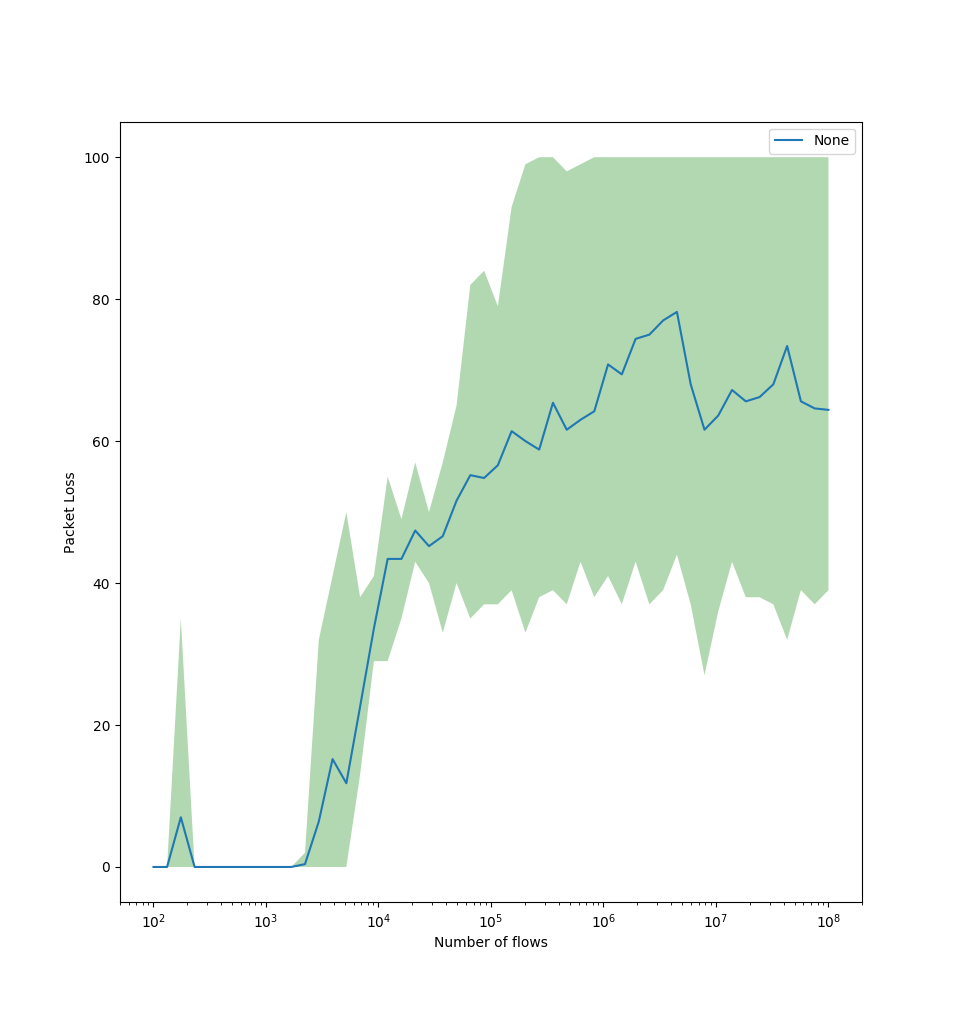
\includegraphics[width=0.5\textwidth]{meter_eleph/ovs_packet_loss}
    \caption {OVS measured packet loss}
    \label{fig:ovs_packet_loss}
\end{figure} 

\section {Algorithm design}

\begin {equation*}
\centering
x_i = 
\begin{bmatrix}
B_{RX}\\
P_{RX}\\
B_{TX}\\
P_{TX}\\
\end{bmatrix}
\end {equation*}

\par $B_{XX}$ and $P_{XX}$ describe to the port statistics obtained from the controller, the byte (B\textsubscript{XX}) and packet (P\textsubscript{XX}) counters, 
respectively, and the indexes describe if the counters account for the transmitted or received data in that port.

\par Using the techniques presented in section \ref{subsec:change_detection}, we build algorithm \ref{alg:high_level}. This is a high level view of the steps
required to obtain the detection, and in the following sections, we introduce each step, and provide some clarifications on the design decisions.

\begin{algorithm}[H]
    \caption{Elephant Detection Algorithm - High Level} \label{alg:high_level}
    \begin{algorithmic}[1]
        \Procedure {Elephant Flow Detection}{}
            \State Initialization
            \State Query controller
            \Loop
                \State Error calculation
                \State Prediction
                \State Detection
                \If {Detection}
                    \State Raise Alarm
                \EndIf
                \State wait 2 seconds
            \EndLoop
        \EndProcedure 
       \end{algorithmic}
\end{algorithm}

\subsection{Initialization}

The initialization step of the algorithm is a crucial step for obtaining correct results in the algorithm. This step allows for the correct initialization of the
model parameters, including the trend component, and to provide a baseline for the expected traffic on the network. Due to these factors, it is assumed that no 
traffic abnormalities exist during this stage, but a longer period for initialization can account for short bursts of higher traffic.

\begin{algorithm}[H]
    \caption{Elephant Detection Algorithm - Initialization} \label{alg:high_level}
    \begin{algorithmic}[1]
        \Procedure {Initialization}{}
            \State initialization period = 30s
            \While {t <= initialization period}
                \State x = Query controller
                \State initialization measures += x
                \State Determine prediction
            \EndWhile
            \State Linear Regression (initialization measures)
        \State \Return Linear regression coefficient
    \end{algorithmic}
\end{algorithm}

\par Detrending the data using the linear regression function comes from the fact that on the end of the initialization period, plotting the received bytes results
in figure \ref{fig:init_plot}.

% Display initial graph of Received Bytes
\begin{figure} 
    \centering
    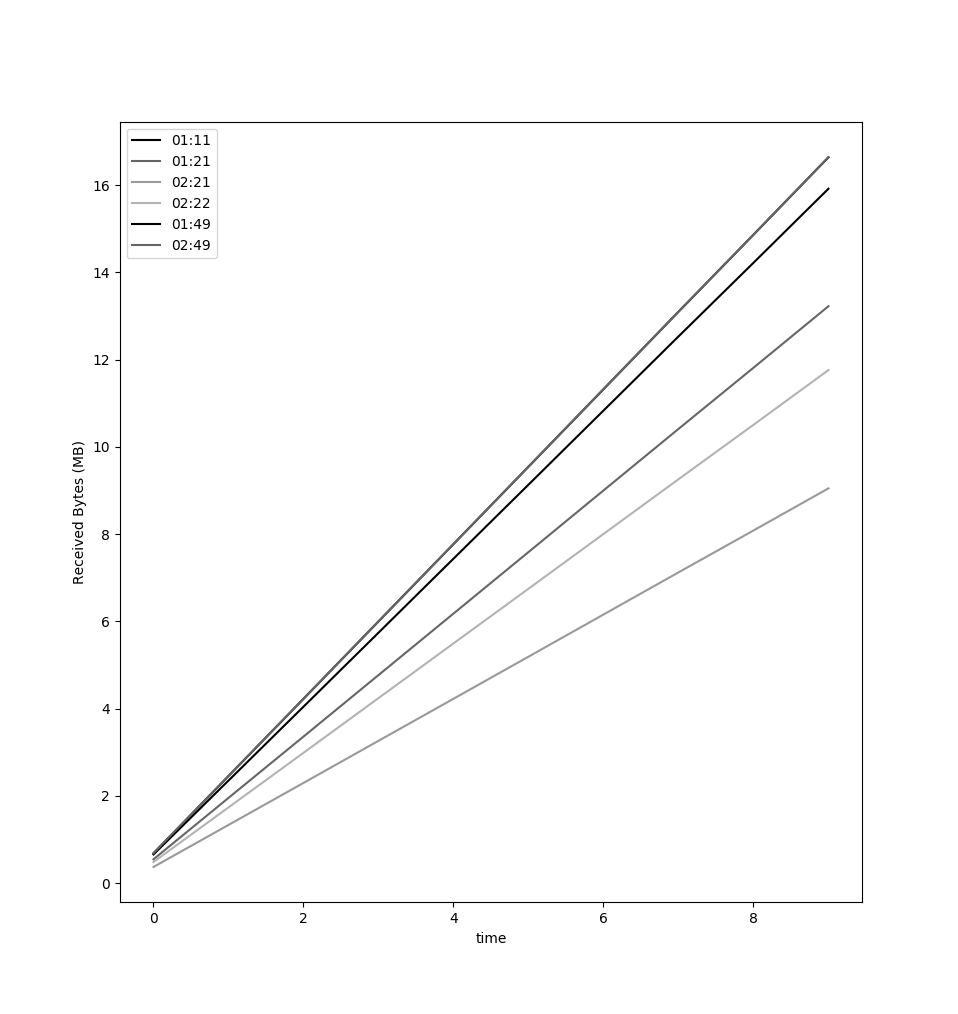
\includegraphics[width=0.4\textwidth]{meter_eleph/init_period_lin}
    \caption {Plotting the initial measurements of B\textsubscript{RX}}
    \label{fig:init_plot}
\end{figure} 

\subsection{Prediction and error calculation}

Using the methods presented in \ref{sec:change_detection}, we are able to predict the values that are expected in the following sample, and determine the error of
the prediction. In this step, the most important consideration is the adjustment of the $\alpha$ parameter, to determine the impact of the variation of
this parameter.

\par Calculating the error was initially determined as

\begin{equation}
    \centering
    \label{eq:division}
    \epsilon = (x_i(t)/\hat{x}_i(t))^2,
\end{equation}

\par which provided the result present in figure \ref{fig:error_plot_division_sse}, and while it clearly indicates the deviations created by the elephant flows, it 
does not provide insight to the level of change caused by higher data sizes in the flows.

Due to this result, we assume higher ($\alpha \rightarrow 1$) values for the smoothing factor for posterior results. A different approach was devised,
and to obtain the values for the error calculation we consider the SSE (\ref{eq:sse}) to increase the impact of larger changes to the flow data size,
and minimize smaller changes.

\begin{figure} [H]
    \centering
    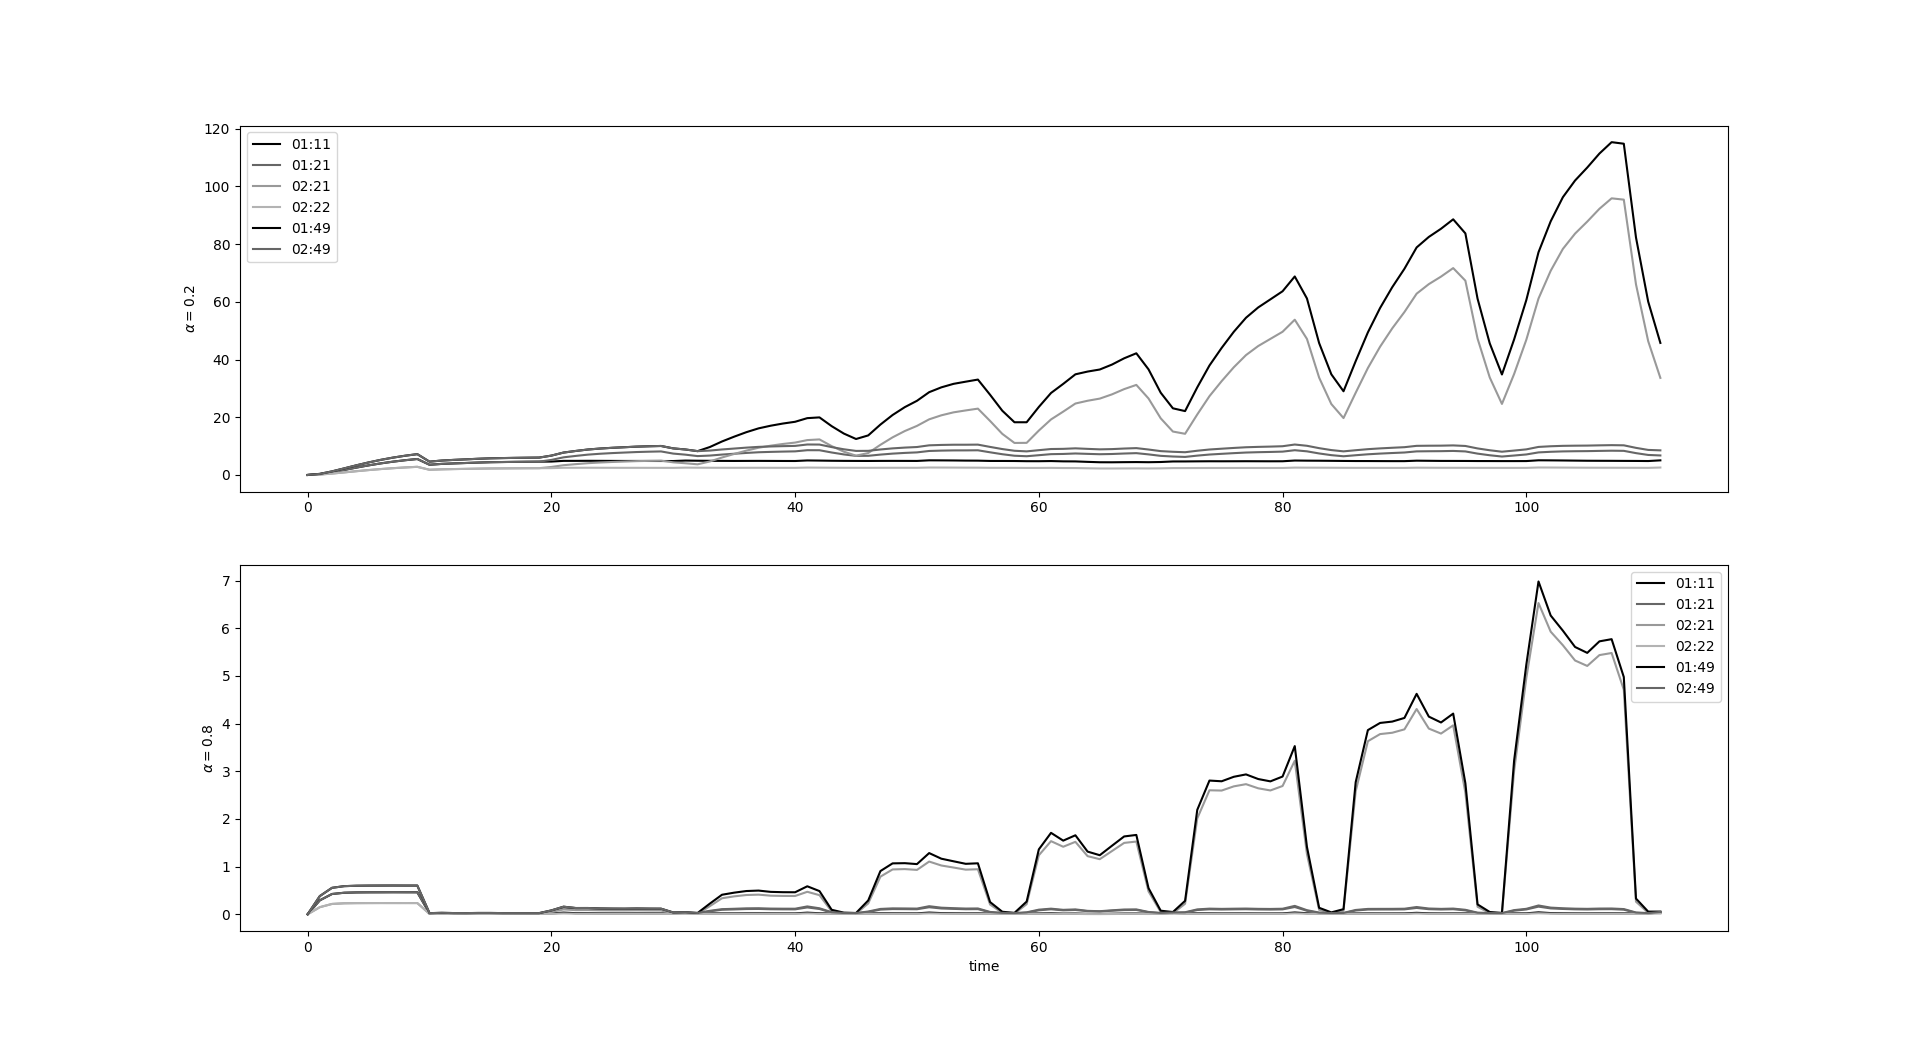
\includegraphics[width=0.7\textwidth]{meter_eleph/error_plot_sse}
    \caption{Different error calculation methods, on the top using SSE, and on the bottom using equation 8.1}
\end{figure}

\subsection{Detection}

The detection component of the algorithm provides the logic for finding the points that are out of control. For this component we consider two possible techniques:
the first, which simply compares the output of the error calculation, to a certain threshold; and a second, using the CUSUM algorithm. 

\par For the first detection method, the rule is 

\begin{equation*}
    \centering
    \label{eq:division}
    \epsilon^2 \geq \delta,
\end{equation*}

\par and this method provides advantages mainly due to the simplicity of the technique, however previous knowledge of the change is required to determine a possible
threshold $\delta$. After cross examining the plots for the decrease of bandwidth, \ref{fig:bandwidth_loss} and the error predictions plots, we assume $\delta = 3$
for the threshold value. The change detection algorithm applied to port 21 can be seen in figure \ref{fig:detect_dumb}.

\begin{figure}[H]
    \centering
    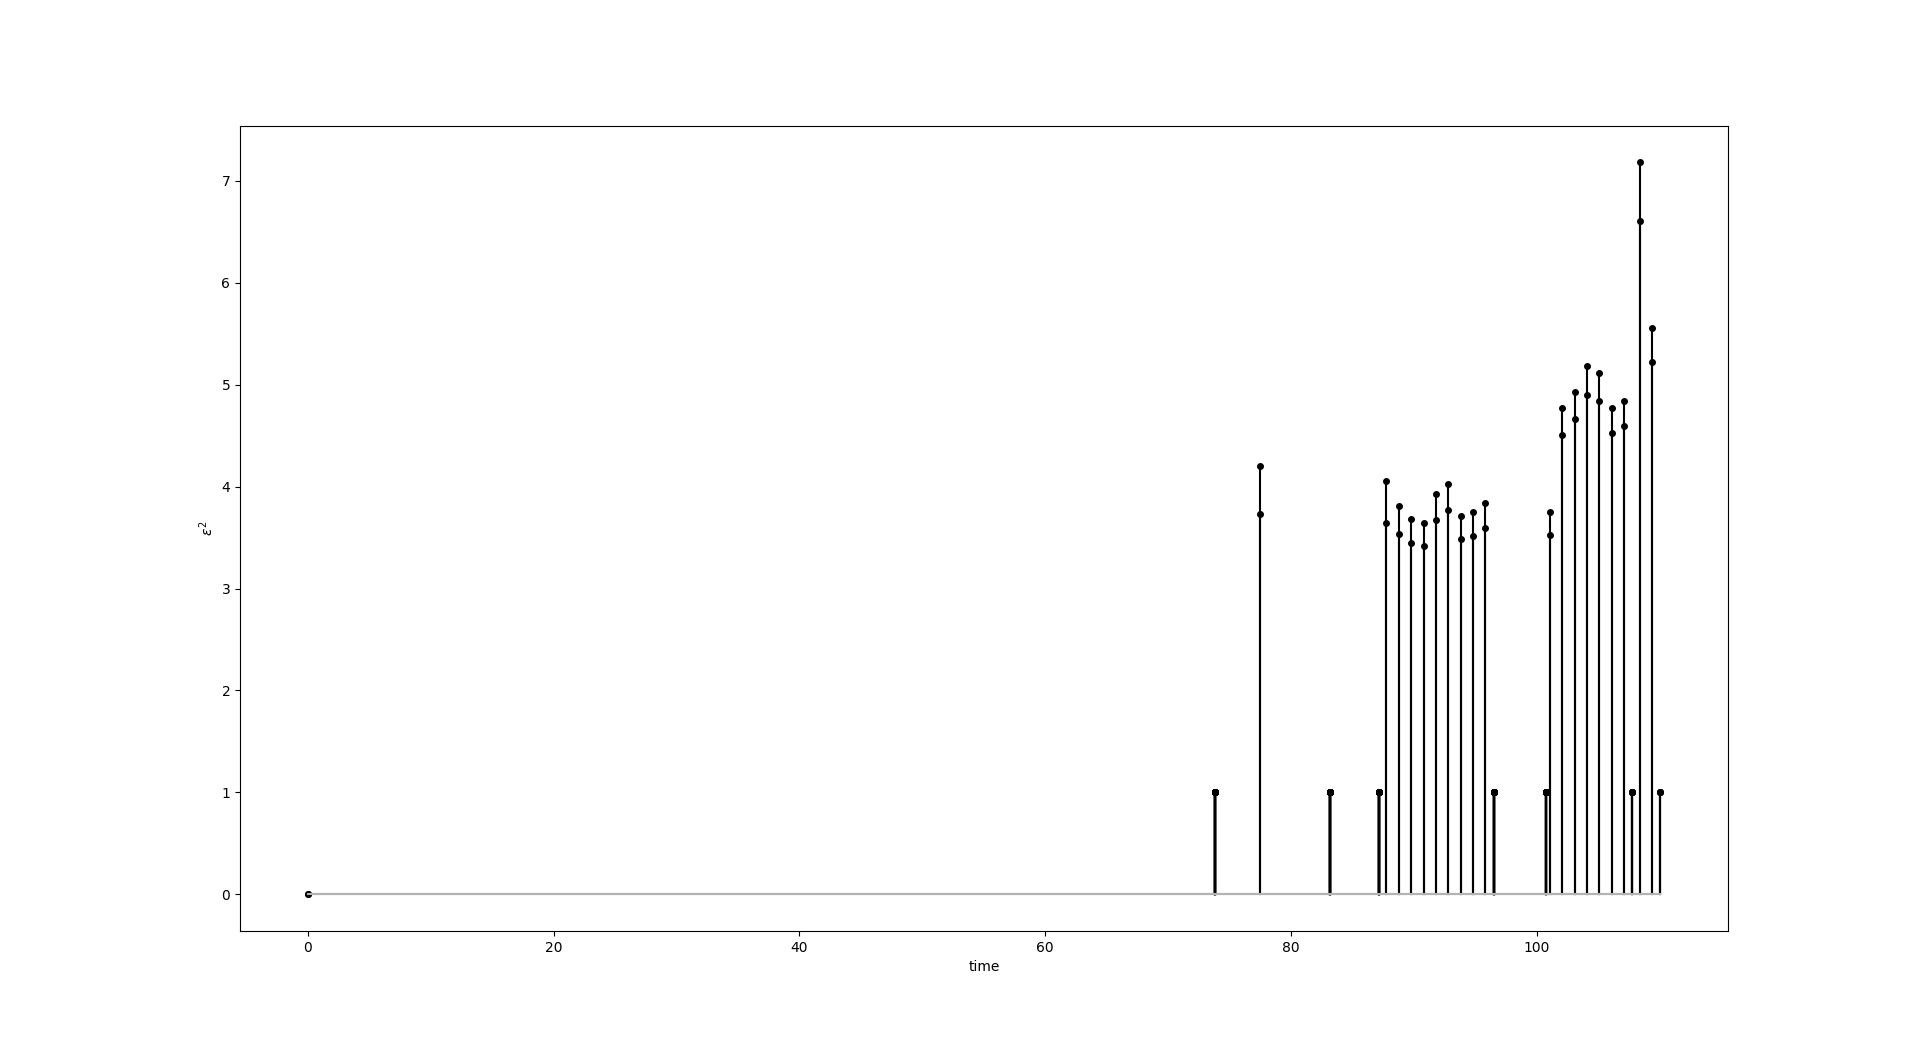
\includegraphics[width=0.8\textwidth]{meter_eleph/detect_dumb}
    \caption {Simple detection}
    \label{fig:detect_dumb}
\end{figure} 

\par Prior to deploying the CUSUM algorithm, in order to obtain the best-case scenario of the detection algorithm, we have collected the results for the prediction
result, and applied the algorithm to the entire generated data set. Performing this step allows to obtain a general knowledge on the expected output of the algorithm,
more specifically the expected number of alarms that are raised in a certain testing environment, so that application of the online algorithm may provide the
closest possible results to the optimal offline version. Figure  \ref{fig:offline_cusum} shows the output of the algorithm applied to the errors associated to
port 21's errors, which is connected to the host that generates the elephant flows, and the CUSUM algorithm implementation used was from 
\url{https://github.com/demotu/BMC}.

% XXX - Explain drift and threshold parameters
\begin{figure} [H]
    \centering
    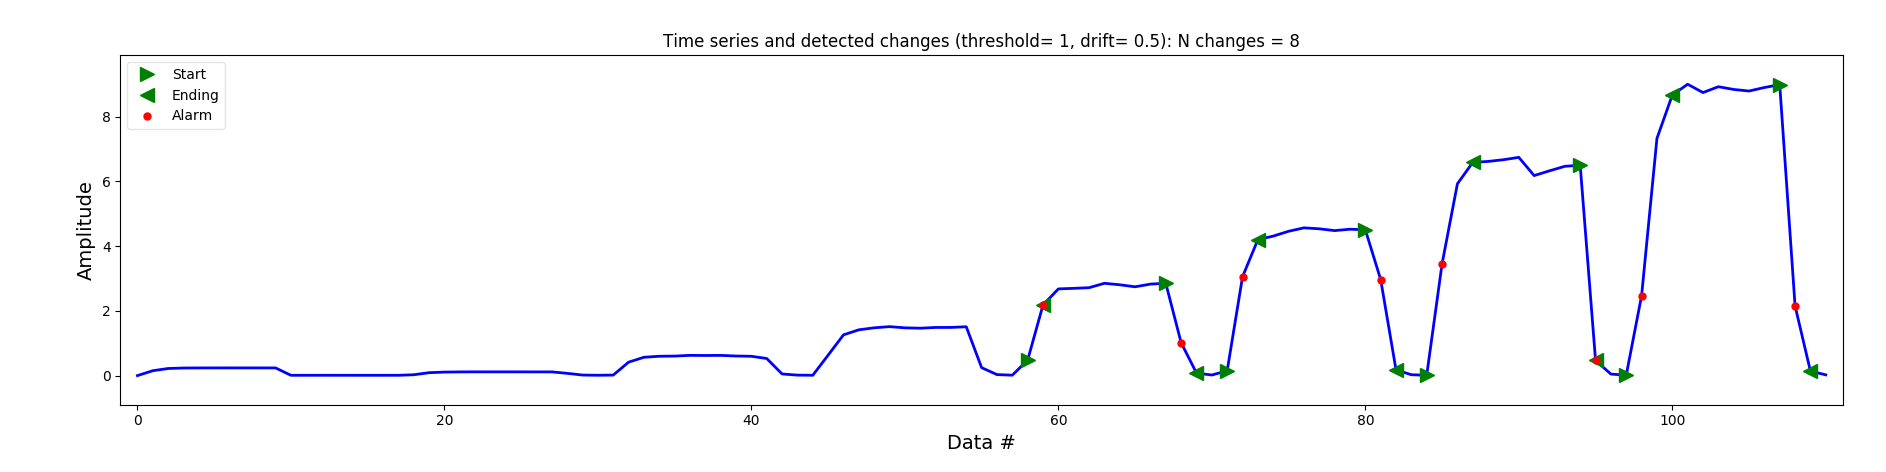
\includegraphics[width=0.8\textwidth]{meter_eleph/offline_cusum_output}
    \caption {Offline CUSUM output}
    \label{fig:offline_cusum}
\end{figure} 

\par The adaptation of the CUSUM algorithm for utilization as an online technique is based on a sliding window that is updated with every new sample. Applying this
method has the advantages of using the CUSUM algorithm without needing extensive changes, while also reducing the amount of memory needed to apply this method. 
Choosing the window size is a central point to a successful implementation of the change detection mechanism, that is explored further in section 
\ref{sec:change_results}. Figure \ref{fig:online_cusum} displays the output of the online CUSUM algorithm in the same testing conditions as the ones present on
the previous results. The points present in this figure are the time when the alarms are raised in relation to the time when the tests began.

\begin{figure} [H]
    \centering
    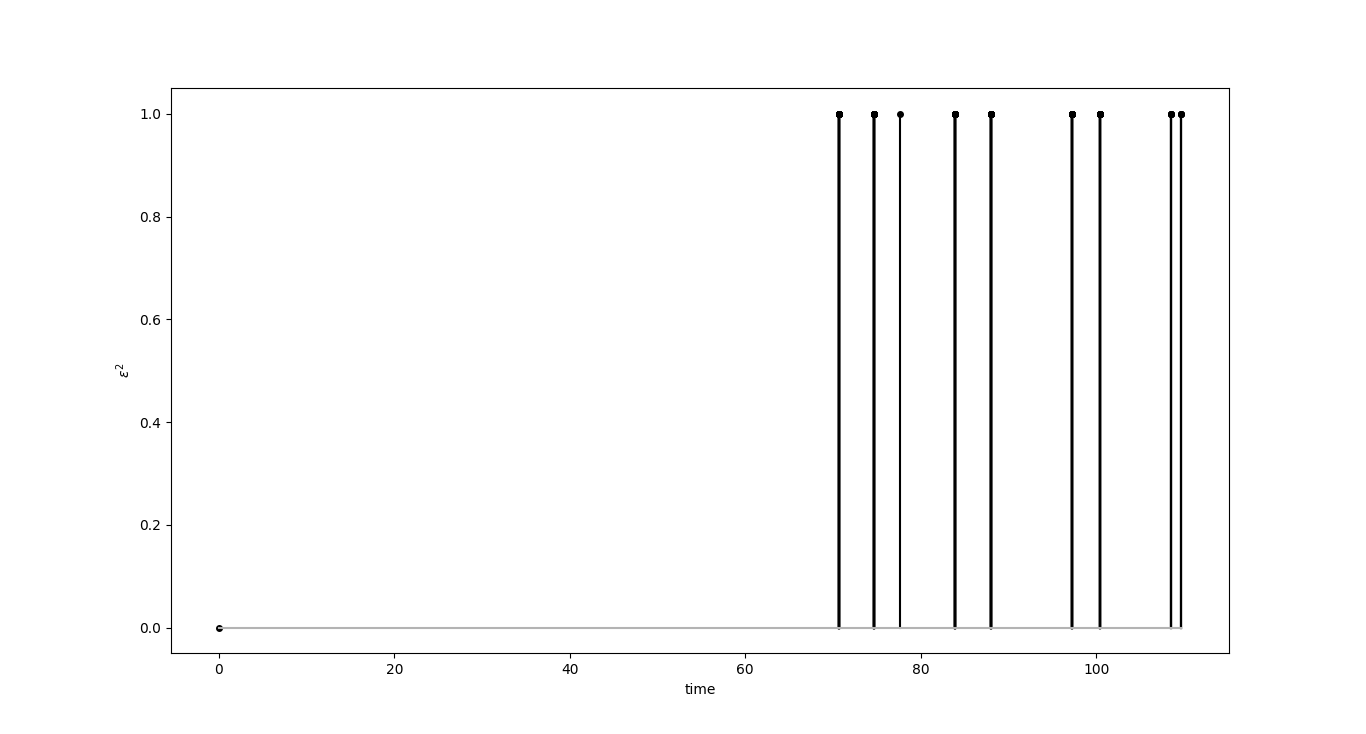
\includegraphics[width=0.8\textwidth]{meter_eleph/online_cusum_output}
    \caption {Online CUSUM output}
    \label{fig:online_cusum}
\end{figure} 

\section {Results and Evaluation} \label{sec:change_result}

Analysing the output of the algorithm provides the information that 

\begin{figure} [H]
    \centering
    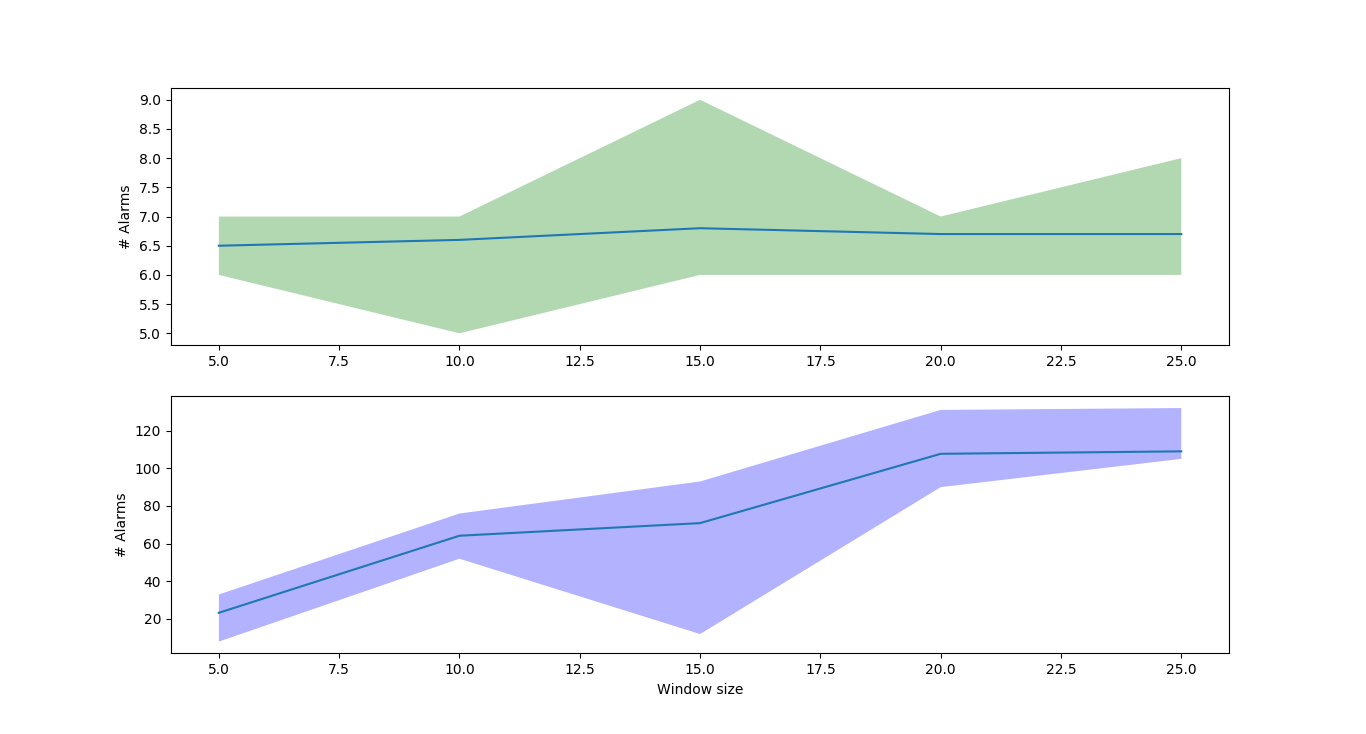
\includegraphics[width=0.8\textwidth]{meter_eleph/evaluation_error}
    \caption {Number of errors comparison between optimized and non optimized version}
    \label{fig:errors_comparaison}
\end{figure} 
